\documentclass[a4paper]{report}

\def\baselinestretch{1.1}
\usepackage[14pt]{extsizes}
\usepackage[utf8]{inputenc}
\usepackage[russian]{babel}
\usepackage{indentfirst}
\usepackage{mathrsfs}

%%%%%%%%%%%%%%%%% Символы, графика %%%%%%%%%%%%%%%%%%%%%

\usepackage[T2A]{fontenc}
\usepackage{amsmath,amssymb,amsfonts,amsthm}
\usepackage{graphicx}
\usepackage{color}
\usepackage[pdftex,colorlinks,linkcolor=blue,citecolor=blue]{hyperref}
\usepackage{pgfplots}
\usepackage{tikz}

%%%%%%%%% Разметка страницы %%%%%%%%%

\usepackage{indentfirst}
\topmargin=-1.5cm %отступ сверху
\oddsidemargin=0.4cm %отступ слева (нечетные страницы)
\evensidemargin=0.4cm %(четные страницы)
\textwidth=16cm %ширина текста
\textheight=24cm
\tolerance=800
\parskip=1ex

\pagestyle{plain}

\usepackage{listings}

\definecolor{codegreen}{rgb}{0,0.6,0}
\definecolor{codegray}{rgb}{0.5,0.5,0.5}
\definecolor{codepurple}{rgb}{0.58,0,0.82}
\definecolor{backcolour}{rgb}{0.95,0.95,0.92}

\lstset{
    backgroundcolor=\color{backcolour},
    commentstyle=\color{codegreen},
    keywordstyle=\color{magenta},
    numberstyle=\tiny\color{codegray},
    stringstyle=\color{codepurple},
    breakatwhitespace=false,
    breaklines=true,
    captionpos=b,
    keepspaces=true,
    numbers=left,
    numbersep=3pt,
    showspaces=false,
    showstringspaces=false,
    showtabs=false,
    tabsize=1,
    basicstyle=\fontsize{10}{12}\selectfont\ttfamily
}

\begin{document}

\begin{titlepage}
	\begin{center}
		Министерство науки и высшего образования РФ\\
		ФГБОУ ВО «Тверской государственный университет»\\
		Математический факультет\\
		Направление 02.03.01 Математика и компьютерные науки\\
		Профиль <<Математическое и компьютерное моделирование>>	
	\end{center}
	
	\vspace{2.5cm}
	\begin{center}
	
		{ВЫПУСКНАЯ КВАЛИФИКАЦИОННАЯ РАБОТА }
		
		
		\vspace{1.0cm}
		\large{Программирование квантовых случайных блужданий}
		
		
		\vspace{1.5cm}
	\end{center}
	
	
	
	\begin{flushright}
		\begin{minipage}{80mm}
			Автор:\\
			Соловьев Илья Олегович
			
			\vspace{1.0cm}
			Научный руководитель:\\
			д. ф.-м. н. Цирулёв А.Н.
			
		\end{minipage}
	\end{flushright}
	
	
	\vspace{1.6cm}
	\noindent Допущен к защите:\\
	Руководитель ООП:\\[1cm]
	\underline{\qquad \qquad \qquad \qquad \qquad }
    В.П. Цветков \\
	\vspace{2.3cm}
	
	
	
	\begin{center}
		Тверь 2022
	\end{center}
	
	\date{}
\end{titlepage}

\setcounter{page}{2}

\tableofcontents
\newpage

% Abstract
\addcontentsline{toc}{chapter}{\hspace{7mm} Введение}


\section*{Введение}

В данной работе изучаются квантовые случайные блуждания на прямой с дискретным временем.
Впервые понятие «Случайное блуждание» было введено английским математиком Карл Пирсон в 1905 году.
Теория случайных блужданий используется в разных областях. Но большую популярность эта теория приобрела в естественных науках, однако встречается и в других сферах.

С появлением у компьюторов больших вычислительных мощностей стало актуальным использование стохастически= методов для решения практических задач -
это объясняет актуальность данной работы. Целью работы является изучение теории классических и квантовызх случайных блужданий, а также их моделирование для .... Для достижения этих целей были поствлены задачи: изучение учебной и научной литературы, разбор принципа классических и квантовых случайных блужданий, составление программ на языке программирования RUST.

Работа состоит из двух глав, заключения и списка литературы. Первая глава носит вводный и обзорный характер. В ней рассматриваются основные принципы классических случайных блужданий на решеткаъ,  связь случайных блужданий с цепями маркова и основные принципы  квантовых случайных блужданий . Во второй главе исследуются квантовые случайные блуждания на примерах. В заключении сформулированы основные результаты работы. Список литературы состоит из 5 источников.


%####################################################
%################# Глава 1 ##################
%####################################################

\chapter{Квантовые блуждания на решетках}

%####################################################

\section{Случайные блуждания на прямой}

Популярной моделью случайного блуждания является модель случайного блуждания по решетке, где на каждом шаге местоположение переходит к другому в соответствии с некоторым распределением вероятностей. При простом случайном блуждании местоположение может переходить только к соседним узлам решетки. В классическом симметричном случайном блуждании по конечной решетке вероятности перехода местоположения к каждому из его непосредственных соседей одинаковы. Если пространство состояний ограничено конечными размерами, модель случайного блуждания называется простым симметричным случайным блужданием с границами, а вероятности перехода зависят от местоположения состояния, поскольку в краевых и угловых состояниях движение ограничено.

Рассмотрим  простейшую математическую модель случайного блуждания. пусть в дискретные моменты времени $t_{0}, t_{1}, ...$ частица может совершить только один скачок вдоль прямой так, что в момент времени $t_{n+1}$, она отстает от точки $t_{n}$ влево или вправо на единичное расстояние. Пусть координата частицы в любой момент времени есть число. Введем на прямой начало отсчета (для удобства возьмем 0, как начало отсчета)

Блуждание имеет случайный характер: с вероятностью $p$ частица может совершить прыжок в права, тогда с вероятностью $q = 1 - p$ частица будет выполнять прыжок влево. В данной случае любые другие перемещения невозможны, так как $p + q = 1$. Отметим, что состояние частицы в момент времени $t_{n+1}$ зависит только от состояния частицы в момент времени $t_{n}$.

Для анализа случайных блужданий удобно пользоваться понятием "случайной" траектории на $n$ шагов.Это набор точек $(j, \xi_{j}), j=0,1...n$ на двумерной плоскости, где первая координата - момент времени $t=j$, а вторая - координата частицы в момент времени $t=j$. Для удобного визуального восприятия удобно соединить точки траектории отрезками прямых, тогда на графики мы увидим непрерывную ломаную из $n$ звеньев. Нам интересно узнать распределения попаданий точек в каждую из координат.

\begin{figure}
  \centering
  % Requires \usepackage{graphicx}
  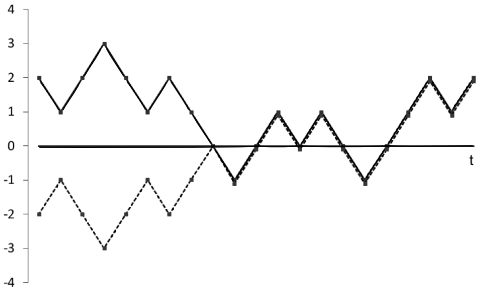
\includegraphics[]{img1.png}\\
  \caption{Ломаная из $n$ звеньев}\label{fig:1}
\end{figure}


\section{Метод цепей Маркова в моделировании случайных блужданий}
Случайные блуждания можно сформулировать по разному. Обычно мы говорим, что случайные блуждания - это последовательность движений, сгенерированных стохастическим (случайным) образом внутри заданного состояния.
Если стохастические движения коррелируют во времени, мы говорим о немарковских блужданиях (блуждания с памятью), однако дальше мы будем говорить только о марковских блужданиях - случайные движения частицы не зависят от времени.
Стоит отметить, что блуждания могут зависеть от положения. Последовательности таких ходов приводят к так называемые цепям Маркова.

Рассмотрим марковский процесс с дискретным временем, в котором вероятности не зависят от номера шага. Общий вид:

\begin{equation} \label{eq:1}
    p^{(k+1)} = p^{(k)}P,
\end{equation}

где $p^{(k)}$ - распределение вероятностей на $k$-ом шаге, а $P$ - матрица переходных вероятностей.

\begin{equation} \label{eq:2}
    ( ... p_{n_{1}}, p_{n_{2}}, p_{n_{3}}, ... )^{(k+1)} = ( ... p_{n_{1}}, p_{n_{2}}, p_{n_{3}}, ... )^{(k)}\left(
                                                                                                               \begin{array}{ccccc}
                                                                                                                 ... & ... & ... & ... & ... \\
                                                                                                                 ... & p_{n_{1}n_{1}} & p_{n_{1}n_{2}} & p_{n_{1}n_{3}} & ... \\
                                                                                                                 ... & p_{n_{2}n_{1}} & p_{n_{2}n_{2}} & p_{n_{2}n_{3}} & ... \\
                                                                                                                 ... & p_{n_{3}n_{1}} & p_{n_{3}n_{2}} & p_{n_{3}n_{3}} & ... \\
                                                                                                                 ... & ... & ... & ... &... \\
                                                                                                               \end{array}
                                                                                                             \right)
    ,
\end{equation}

где $... p_{n_{1}}, p_{n_{2}}, p_{n_{3}}, ... $ - вероятности нахождения частицы в точках $..., n_{1}, n_{2}, n_{3}, ...$ на $k$-ом шаге. Для любой строки матрицы $P$ элементы $p_{ij} > 0$, сумма элементов в строке должна равняться 1. $p_{ij}$ - вероятность перейти в позицию $j$ при условии, что на $k$ шаге мы находились в позиции $i$.

Имея матрицу $P$ и начальное состояние $( ... p_{n_{1}}, p_{n_{2}}, p_{n_{3}}, ... )^{(0)}$, распределение после m шагов описывается уравнением:

\begin{equation} \label{eq:2}
    ( ... p_{n_{1}}, p_{n_{2}}, p_{n_{3}}, ... )^{(m)} = ( ... p_{n_{1}}, p_{n_{2}}, p_{n_{3}}, ... )^{(0)} P^{m}
    ,
\end{equation}

Для примера возьмем случайное блуждание на целочисленном отрезке $[-2, 2] \subset \mathbb{Z}$, тогда получим:

\begin{equation} \label{eq:3}
    ( p_{-2}, p_{-1}, p_{0}, p_{1}, p_{2})^{(k+1)} = ( p_{-2}, p_{-1}, p_{0}, p_{1}, p_{2})^{(k)} \left(
                                                                                                    \begin{array}{ccccc}
                                                                                                      q & p & 0 & 0 & 0 \\
                                                                                                      q & 0 & p & 0 & 0 \\
                                                                                                      0 & q & 0 & p & 0 \\
                                                                                                      0 & 0 & q & 0 & p \\
                                                                                                      0 & 0 & 0 & 1 & 0 \\
                                                                                                    \end{array}
                                                                                                  \right)
    ,
\end{equation}


\section{Квантовые случайные блуждания}

Квантовые блуждания — это квантовые аналоги классических случайных блужданий. Они также как и в случае с классическими случайными блужданиями делятся на два типа: непрерывные и дискретные(далее будут рассматриваться дискретниые). В отличие от классического случайного блуждания, где частица принимает  определенные состояния, а случайность возникает за счет стохастических переходов между состояниями, в квантовых блужданиях случайность возникает за счет: квантовой суперпозиции состояний, неслучайной обратимой унитарной эволюции. Характерным свойством квантовых случайных блужданий является локализация, которая определяется тем, что вероятность того, что частица окажется в точке, не сходится к нулю даже в пределе больших времен.

Квантовые блуждания мотивированы широким использованием классических случайных блужданий при разработке рандомизированных алгоритмов и являются частью нескольких квантовых алгоритмов. Для некоторых задач оракула
\footnote{
В теории вычислимости машина-оракул — это абстрактная машина, используемая для изучения проблем принятия решений. Его можно представить как машину Тьюринга с черным ящиком, называемым оракулом, который способен решать определенные задачи за одну операцию. Задача может быть любого класса сложности. Можно использовать даже неразрешимые проблемы, такие как проблема остановки.}
квантовые блуждания обеспечивают экспоненциальное ускорение по сравнению с любым классическим алгоритмом. Квантовые блуждания также дают полиномиальное ускорение по сравнению с классическими алгоритмами для многих практических задач, таких как проблема уникальности элементов, проблема поиска треугольников. Известный алгоритм поиска Гровера также можно рассматривать как алгоритм квантового блуждания.

Далее  мы сосредоточимся на пространственно-неоднородных квантовых блужданий в одномерном пространстве. В качестве простых случаев мы рассматривать квантовые блуждания, вызванные блужданием Адамара.
% Сделать тут все определениями и добавить определение амплитуды
Кубит — наименьшая единица информации в квантовом компьютере (аналог бита в обычном компьютере), использующаяся для квантовых вычислений.
Как и бит, кубит допускает два собственных состояния, обозначаемых $|0\rangle$ и $|1\rangle$, но при этом может находиться и в их суперпозиции. В общем случае его волновая функция имеет вид $A|0\rangle + B|1\rangle$ где $A$ и $B$ амплитудами вероятностей и являются комплексными числами, удовлетворяющими условию $|A|^{2} - |B|^{2} = 1$.
При измерении состояния кубита можно получить лишь одно из его собственных состояний. Вероятности получить каждое из них равны  $|A|^{2}$ и $|B|^{2}$ соответственно.

Квантовый вентиль (квантовый логический элемент) — это базовый элемент квантового компьютера, преобразующий входные состояния кубитов на выходные по определённому закону. Отличается от обычных логических вентилей тем, что работает с кубитами. Квантовые вентили в отличие от многих классических всегда являются обратимыми.

Так как кубит можно представить вектором в двумерном пространстве, то действие вентиля можно описать унитарной матрицей, на которую умножается соответствующий вектор состояния входного кубита. Однокубитные вентили описываются матрицами размера $2 \ast 2$,
двухкубитные — $4 \ast 4$, а $n$-кубитные — $2^{n} \ast 2^{n}$.

Примеры простейших однокубитовых вентилей:
\begin{itemize}
  \item Тождественное преобразование

    $$
        \left(
          \begin{array}{cc}
              1 & 0 \\
              0 & 1 \\
          \end{array}
        \right)
    $$

  \item Отрицание

  $$
        \left(
          \begin{array}{cc}
              0 & 1 \\
              1 & 0 \\
          \end{array}
        \right)
  $$

  \item Преобразование Адамара

  $$
        \frac{1}{\sqrt{2}}
        \left(
          \begin{array}{cc}
              1 & 1 \\
              1 & -1 \\
          \end{array}
        \right)
  $$

\end{itemize}


%####################################################
%################# Глава 2 ##################
%####################################################


\chapter{Моделирование квантовых случайных блужданий}



%####################################################

\section{Правила перехода}

В классических случайных блужданиях на прямой мы начинали с позиции 0. На каждом шаге мы имели возможность переместиться влево или вправо с одинаковой вероятностью. В квантовых случайных блужданиях аналогом будет квантовый процесс с базисными состояниями
$|n\rangle, n \in \mathbb{Z} $. На каждом временном шаге он будет выполнять преобразование
\begin{equation} \label{eq:3}
    |n\rangle \rightarrow a|n - 1\rangle +  b|n\rangle + c| n + 1\rangle
\end{equation}
что означает движение влево с амплитудой $a$ сохранение позиции с амплитудой $b$ и движение вправо с амплитудой $c$.Также мы хотели бы, чтобы движение осуществлялось в каждую из сторон. Т.е. $a, b, c$ не должны зависеть от шага(так же, как и в классических блужданиях перемещение влево/вправо не зависят от шага $n$). Но в данном случае так не выйдет.

Преобразование $U$, определяемое уравнением ~(\ref {eq:1}) является унитарным тогда и только тогда, когда выполняется одно из следующих условий:

\begin{enumerate}
     \item |a|  =  1, b = c = 0;
     \item |b|  =  1, a = c = 0;
     \item |c|  =  1, a = b = 0;
\end{enumerate}

Из этого мы можем сделать вывод, что единственно возможными преобразованиями является тривиальные (те, при которых движение возможно только в одну из сторон, либо остановка на месте).

Эту проблему можно решить введя дополнительное "монетное" состояние. Мы будем рассматривать пространство из состояний  $|n, 0\rangle$ и $|n, 1\rangle$  при $n  \in \mathbb{Z} $. На каждом шаге мы будем выполнять две операции:

%"Трансформация подбрасывания монеты" С: - назвать по нормальному, звучит плохо

\begin{enumerate} \label{qbit_transformation}
     \item $C|n, 0\rangle = a|n, 0\rangle + b|n, 1\rangle$
     \item $C|n, 1\rangle = c|n, 0\rangle + d|n, 1\rangle$
\end{enumerate}

Сдвиг S:
\begin{equation} \label{coin_transformation}
    S|n, 0\rangle = |n - 1, 0\rangle, S|n, 1\rangle = |n + 1, 1\rangle
\end{equation}

Шаг квантового блуждания - это $SC$. Для $C$ часто выбирают преобразование Адамара:

\begin{equation} \label{eq:1}
\begin{pmatrix}
  a& b \\
  c& d
\end{pmatrix}
=
\begin{pmatrix}
  \frac{1}{\sqrt{2}} & \frac{1}{\sqrt{2}} \\
  \frac{1}{\sqrt{2}}& -\frac{1}{\sqrt{2}}
\end{pmatrix}
\end{equation}

Можно использовать любое другое двумерное унитарное преобразование.

Можно думать о $C$ как о квантовом аналоге подбрасывания монетки, в котором мы решаем, в каком из направлений мы будем двигаться. Чтобы разобраться с тем, как это работает, мы рассмотрим пример, в котором между $C$ и $S$ мы измерим состояние.  Если состояние до C было равно $|n, 0\rangle$, то после состояние будет равно
$\frac{1}{\sqrt{2}} |n,0\rangle + \frac{1}{\sqrt{2}}|n,1\rangle$ и измерение этого выражения дает нам $|n,0\rangle$ и $|n,1\rangle$ с вероятностью $0.5$ для каждого.Таким оразом мы видим, что $C$ эквивалентно выбору одного кубита из $|n,0\rangle$ и $|n,1\rangle$ с вероятностями $0.5$ для каждого.

Рассмотрим три первых шага квантового блуждания с преобразованием Адамара с начальным состоянием $|0, 0\rangle$:

\begin{enumerate}
     \item $|0, 0\rangle \rightarrow$
     \item $\frac{1}{\sqrt{2}}|0, 0\rangle + \frac{1}{\sqrt{2}}|0, 1\rangle \rightarrow \frac{1}{\sqrt{2}}|-1, 0\rangle + \frac{1}{\sqrt{2}}|1, 1\rangle \rightarrow$
     \item $\frac{1}{2}|-1, 0\rangle + \frac{1}{2}|-1, 1\rangle + \frac{1}{2}|1, 0\rangle - \frac{1}{2}|1, 1\rangle \rightarrow \frac{1}{2}|-2, 0\rangle + \frac{1}{2}|0, 1\rangle + \frac{1}{2}|0, 0\rangle - \frac{1}{2}|2, 1\rangle \rightarrow$
     \item $\frac{1}{2\sqrt{2}}|-2, 0\rangle + \frac{1}{2\sqrt{2}}|-2, 1\rangle + \frac{1}{\sqrt{2}}|0, 0\rangle - \frac{1}{2\sqrt{2}}|2, 0\rangle + \frac{1}{2\sqrt{2}}|2, 1\rangle \rightarrow \frac{1}{2\sqrt{2}}|-3, 0\rangle + \frac{1}{2\sqrt{2}}|-1, 1\rangle + \frac{1}{\sqrt{2}}|-1, 0\rangle - \frac{1}{2\sqrt{2}}|1, 0\rangle + \frac{1}{2\sqrt{2}}|3, 1\rangle$
\end{enumerate}

%####################################################

\section{Случайные возмущения процесса}

Нужна помощь с написанием вступления в этой главе(для чего это делается)

Квантовым вентелем может быть любая матрица $A$ определяемая как:
\begin{equation}
   A = \left(
      \begin{array}{cc}
        a_{0}+ i a_{3} & -a_{1} + i a_{2} \\
        a_{1} + i a_{2} & a_{0} - i a_{3} \\
      \end{array}
    \right)
\end{equation}

При условии, что:

\begin{enumerate}
  \item $a_{0}^{2} + a_{1}^{2} + a_{2}^{2} + a_{3}^{2} = 1$
  \item $A^{*} * A = E$
\end{enumerate}

Для дальнейщего моделирования квантового блуждания введем слежущее возмущение процесса: пусть $p \in [0, 1)$ - число, которое случайным образом генирируется перед каждым преобразованием. В случае когда $p > 0.9$ мы будем выполнять следущее преобразование:

\begin{equation} \label{disturbance_transformation}
   \left(
      \begin{array}{cc}
       \sqrt{p} & -\sqrt{1 - p} \\
       \sqrt{1 - p} & \sqrt{p} \\
      \end{array}
    \right)
\end{equation}

%####################################################

\section{Математические модели и алгоритмы простейших квантовых случайных блужданий}

Алгоритм реализован на языке программирования Rust. Он был выбран из-за скорости его работы, довольно удобного синтаксиса (позволяет разрабатывать как в функциональном так и объектно-ориентированном стиле) и компилятора.

Для начала нужно реализовать дополнительные функции для того, чтобы код был самодокументируемым и простым в расширении.
Начнем с создания структуры Qbit.
\begin{lstlisting}
    struct Qbit {
        amplitude: f64,
        position: i32,
        coin_state: bool,
    }
\end{lstlisting}

\begin{itemize}
  \item амплитуда
  \item точка в которой может находиться наша частица
  \item монетное состояние
\end{itemize}

Добавим "вспомогательные"  функции:
\begin{itemize}
  \item \begin{verbatim}hadamar(initial_qbit: &Qbit) -> (Qbit, Qbit)\end{verbatim} - преобразование Адамара
  \item \begin{verbatim}coin_transformation(initial_qbit: Qbit) -> Qbit\end{verbatim}  - трансформация подбрасывания монеты, которая ранее была названа, как S
  \item \begin{verbatim}get_qbit_key(position: i32, coin_state: bool) -> String\end{verbatim} - получение уникального ключа для каждого кубита
  \item \begin{verbatim}unit_transformation(initial_qbit: &Qbit, p: f64) -> (Qbit, Qbit)\end{verbatim} - реализация ~(\ref {disturbance_transformation})
\end{itemize}

Рассмотри подробнее каждую из этих функций c комментариями.
\begin{lstlisting}
fn hadamar(initial_qbit: &Qbit) -> (Qbit, Qbit) {
  return if initial_qbit.coin_state == false {
    (
      Qbit {
        amplitude: initial_qbit.amplitude * (1.0 / 2_f64.sqrt()),
        position: initial_qbit.position,
        coin_state: false,
      },
      Qbit {
        amplitude: initial_qbit.amplitude * (1.0 / 2_f64.sqrt()),
        position: initial_qbit.position,
        coin_state: true,
      })
  } else {
    (
      Qbit {
        amplitude: initial_qbit.amplitude * (1.0 / 2_f64.sqrt()),
        position: initial_qbit.position,
        coin_state: false,
      },
      Qbit {
        amplitude: initial_qbit.amplitude*(1.0 / 2_f64.sqrt()) * -1.0,
        position: initial_qbit.position,
        coin_state: true,
      })
  };
}
\end{lstlisting}
Реализация ~(\ref {qbit_transformation}) c выбранным преобразованием Адамара. На основе исходного кубита, мы получаем два новых с амплитудами, которые зависят от монетного состояния и граничных условий.
\begin{lstlisting}
fn coin_transformation(initial_qbit: Qbit, borders: (i32, i32)) -> Qbit {
  return if initial_qbit.coin_state {
    if initial_qbit.position == borders.1 {
      Qbit {
        amplitude: initial_qbit.amplitude,
        coin_state: initial_qbit.coin_state,
        position: initial_qbit.position - 1,
      }
    } else {
      Qbit {
        amplitude: initial_qbit.amplitude,
        coin_state: initial_qbit.coin_state,
        position: initial_qbit.position + 1,
      }
    }
  } else {
    if initial_qbit.position == borders.0 {
      Qbit {
        amplitude: initial_qbit.amplitude,
        coin_state: initial_qbit.coin_state,
        position: initial_qbit.position + 1,
      }
    } else {
      Qbit {
        amplitude: initial_qbit.amplitude,
        coin_state: initial_qbit.coin_state,
        position: initial_qbit.position - 1,
      }
    }
  };
}
\end{lstlisting}

Релизация ~(\ref {coin_transformation}). В случае, когда монетное состояние равно 1, мы возвращаем новый кубит у которого позиция изменилась на  $n + 1$, в обратном кубит с позицией частицы $n - 1$. Но также стоит сотметить, что в случаае, когда частица находиться на границах, то мы будем перемещать частиуц в противоположную от границы сторону на 1 единицу. За это отвечают строчки 7, 13, 21, 27.

\begin{lstlisting}
    fn get_qbit_key(position: i32, coin_state: bool) -> String {
        coin_state.to_string() + ";" + &*position.to_string()
    }
\end{lstlisting}

Кубит идентифицируют его два состояния - точка в которой находиться частица, монетное состояние. Эта функция нужна, чтобы во время блуждания найти в хеш-таблице кубит с такими же состояниями и пересчитать его амплитуду основываясь на только что полученых новых значения амплитуды.

Перейдем к основной программе.

\begin{lstlisting}
  let mut states: HashMap<String, Qbit> = HashMap::new();
  let borders = (-15, 15);
  let mut rng = rand::thread_rng();
  let mut entropy: f64 = 0.0;
  let mut file = File::create("quantum-walks2.txt").unwrap();
\end{lstlisting}

\begin{itemize}
  \item \textit{states} - хеш-таблица с ключом, созданным с помощью \textit{getQbitKey} и значением - структурой \textit{Qbit}
  \item \textit{entropy} - зачение энтропии
  \item \textit{borders} - кортеж из двух чисел, которые является граничными условиями
  \item \textit{rng} - инстанс структуры rand, которые дает возможность получать случайное число от 0 до 1
  \item \textit{file} - структура с методами записи информации в файл "quantum-walks2.txt"
\end{itemize}

Теперь нужно задать начальные условия $|0, 0\rangle$. Для этого вставим в \textit{states} первое значение.

\begin{lstlisting}
 states.insert(get_qbit_key(0, false), Qbit {
    amplitude: 1.0,
    position: 0,
    coin_state: false,
  });
\end{lstlisting}

\begin{lstlisting}
  for n in (10..=100).step_by(10) {
    for _ in 1..=n {
      let mut temp_states: HashMap<String, Qbit> = HashMap::new();

      let mut insert_qbit_to_hash_map = |key: String, qbit: Qbit| {
        match temp_states.get(&key) {
          None => {
            temp_states.insert(key, qbit);
          }
          Some(currentQbit) => {
            let amplitude: f64 = currentQbit.amplitude + qbit.amplitude;
            if amplitude == 0.0 {
              temp_states.remove(&*key);
            } else {
              temp_states.insert(key, Qbit {
                amplitude: currentQbit.amplitude + qbit.amplitude,
                coin_state: qbit.coin_state,
                position: qbit.position,
              });
            }
          }
        }
      };
      let p = rng.gen::<f32>();

      for state in states.values() {

        let qbits: (Qbit, Qbit);

        if p > 0.9 {
          qbits = unit_transformation(state, p as f64);
        } else {
          qbits = hadamar(state);
        }

        let shiftedFirstQbit = coin_transformation(qbits.0, borders);
        let shiftedSecondQbit = coin_transformation(qbits.1, borders);

        let first_qbit_key = get_qbit_key(shiftedFirstQbit.position, shiftedFirstQbit.coin_state);
        let second_qbit_key = get_qbit_key(shiftedSecondQbit.position, shiftedSecondQbit.coin_state);

        insert_qbit_to_hash_map(first_qbit_key, shiftedFirstQbit);
        insert_qbit_to_hash_map(second_qbit_key, shiftedSecondQbit);
      }

      states = temp_states;
    }


    for state in states.values() {
      let probability = f64::powf(state.amplitude, 2.0);

      if probability != 0.0 {
        entropy -= probability * probability.ln();
      }
    }
    writeln!(&mut file, "n: {} s: {}", n, entropy);

    entropy = 0.0;
  }
\end{lstlisting}

В строках 1-2 мы создаем цикл for, с шагом $n$ в 10 единиц. Количество выполенных преобразований перед вычислением энтропии будут зависеть от $n$.
В 3 строке создадаем временную хеш таблицу в которую мы будем записывать результаты нашего преобразования на каждом шаге.
Строки 5-23 отвечают за замыкание, которое будет добавлять в нашу временнцю хеш таблицу только что полученные кубиты. Давайте детально рассмотрим, как эта функция работает.
Если в нашей таблице еще не существует значения с переданным ключем, то мы просто вставляем это значение в таблциу. Но в случае, когда это значение есть мы вчислаяем амплитуду по формуле $currentQbit.amplitude + qbit.amplitude$. В случае, если это значение равняется нулю, то мы удаляет из таблицы кубит по переданному ключу, но если значение амплитуды не равно нулю, то мы записываем по ключу новы кубит с тоько что вычисленной амплитудой.

На строке 24 создаем переменную p, которая принимает случайным образом значение от 0 до 1. Она отвечает за возмещение процесса, кеоторое было описано в ~(\ref {disturbance_transformation})

В строках 26-47  происходит вычисление состояний кубитов. В 26 строке мы создаем итератор по значения которого мы будем пробегать и на их основе вычислать новые значения кубитов.
На строке 28 создаем новую переменную \textit{qbits}, в которой будет находиться результат унитарного преобразования.
Строки 30-34 отвечают за само унитрное преобразование, в которых с вероятностью $p$ будет выполнение преобразование Адамара, и с вероятностью $1 - p$  преобразование ~(\ref {disturbance_transformation}).
В строках 36-37 мы создадим две перенных \textit{shiftedFirstQbit} и \textit{shiftedSecondQbit}, в которых будут находиться результат "монетного преобразования" первого и второго кубита соответственно.
В строках 42-43 мы вставляем результаты в нашу временную хеш таблицу.

На 46 строке мы записываем значниея, которые хранились во временной хеш таблице в основную. Временная таблица была создана для того, чтобы во вроемя итерации по основной не мутировать ее. В случае, когда бы мы ее мутировали, то у нас этот цикл выполнялся бесконечно, а компилятор Rust даже не дал бы запустить программу из-за утечки памяти.

Строки 50-59 отвечают за вычисление энтропии и записи результата в файл с соотетствующим ей количеством шагов. 

%####################################################

\newpage
\addcontentsline{toc}{chapter}{\hspace{7mm} Заключение}
\section*{Заключение}

В работе получены следующие основные результаты

%####################################################

\newpage
\addcontentsline{toc}{chapter}{\hspace{7mm} Литература}

\begin{thebibliography}{99}

\bibitem{Guld1990}
Х. Гулд, Я. Тобочник. \textit{Компьютерное моделирование в физике. Том\,2}. М.: Мир, 1990

\bibitem{Reitzner2011}
D. Reitzner, D. Nagaj, V. Buzek. \textit{Quantum walks}. Acta Physica Slovaca, \textbf{61}, No.\,6, 2011, pp.\,603\,--\,725
(\href{https://arxiv.org/abs/1207.7283}{\textit{arXiv:} 1207.7283})

\bibitem{Ambainis2004}
A. Ambainis. \textit{Quantum walks and their algorithmic applications}. 2004\\ (\href{https://arxiv.org/abs/quant-ph/040312} {\textit{arXiv:} quant-ph/0403120})

\bibitem{Kempe2003}
J. Kempe. \textit{Quantum random walks --- an introductory overview}. Contemporary Physics, \textbf{44}, Issue 4, 2003, pp. 307\,--\,327\\ (\href{https://arxiv.org/abs/quant-ph/0303081} {\textit{arXiv:} quant-ph/0303081})

\bibitem{Molfetta2021}
G.\,D. Molfetta. \textit{Quantum walks, limits and transport equations, Sec.\,3}. 2021
(\href{https://arxiv.org/abs/2112.11828}{\textit{arXiv:} 2112.11828})

\end{thebibliography}

\newpage
\addcontentsline{toc}{chapter}{\hspace{7mm} Приложение {C\small{$\#$}}, {C\small{$++$}}, Java --- ненужное удалить}

\chapter*{Приложение {\huge Rust}}
\section*{1.\,Программа}

\begin{lstlisting}
use rand::Rng;
use std::fs::File;
use std::io::prelude::*;
use std::collections::HashMap;

struct Qbit {
  amplitude: f64,
  position: i32,
  coin_state: bool,
}

fn main() {
  quantum_walks();
}


fn quantum_walks() {
  let mut file = File::create("quantum-walks2.txt").unwrap();
  let mut states: HashMap<String, Qbit> = HashMap::new();
  let borders = (-15, 15);
  let mut rng = rand::thread_rng();

  let mut entropy: f64 = 0.0;

  states.insert(get_qbit_key(0, false), Qbit {
    amplitude: 1.0,
    position: 0,
    coin_state: false,
  });
  for n in (10..=100).step_by(10) {
    for _ in 1..=n {
      let mut temp_states: HashMap<String, Qbit> = HashMap::new();

      let mut insert_qbit_to_hash_map = |key: String, qbit: Qbit| {
        match temp_states.get(&key) {
          None => {
            temp_states.insert(key, qbit);
          }
          Some(currentQbit) => {
            let amplitude: f64 = currentQbit.amplitude + qbit.amplitude;
          
            if amplitude == 0.0 {
              temp_states.remove(&*key);
            } else {
              temp_states.insert(key, Qbit {
                amplitude: currentQbit.amplitude + qbit.amplitude,
                coin_state: qbit.coin_state,
                position: qbit.position,
              });
            }
          }
        }
      };
      let p = rng.gen::<f32>();

      for state in states.values() {

        let qbits: (Qbit, Qbit);

        if p > 0.9 {
          qbits = unit_transformation(state, p as f64);
        } else {
          qbits = hadamar(state);
        }

        let shiftedFirstQbit = coin_transformation(qbits.0, borders);
        let shiftedSecondQbit = coin_transformation(qbits.1, borders);

        let first_qbit_key = get_qbit_key(shiftedFirstQbit.position, shiftedFirstQbit.coin_state);
        let second_qbit_key = get_qbit_key(shiftedSecondQbit.position, shiftedSecondQbit.coin_state);

        insert_qbit_to_hash_map(first_qbit_key, shiftedFirstQbit);
        insert_qbit_to_hash_map(second_qbit_key, shiftedSecondQbit);
      }

      states = temp_states;
    }


    for state in states.values() {
      let probability = f64::powf(state.amplitude, 2.0);

      if probability != 0.0 {
        entropy -= probability * probability.ln();
      }
    }
    writeln!(&mut file, "n: {} s: {}", n, entropy);

    entropy = 0.0;
  }
}

fn get_qbit_key(position: i32, coin_state: bool) -> String {
  coin_state.to_string() + ";" + &*position.to_string()
}

fn hadamar(initial_qbit: &Qbit) -> (Qbit, Qbit) {
  return if initial_qbit.coin_state == false {
    (
      Qbit {
        amplitude: initial_qbit.amplitude * (1.0 / 2_f64.sqrt()),
        position: initial_qbit.position,
        coin_state: false,
      },
      Qbit {
        amplitude: initial_qbit.amplitude * (1.0 / 2_f64.sqrt()),
        position: initial_qbit.position,
        coin_state: true,
      })
  } else {
    (
      Qbit {
        amplitude: initial_qbit.amplitude * (1.0 / 2_f64.sqrt()),
        position: initial_qbit.position,
        coin_state: false,
      },
      Qbit {
        amplitude: initial_qbit.amplitude * (1.0 / 2_f64.sqrt()) * -1.0,
        position: initial_qbit.position,
        coin_state: true,
      })
  };
}

fn unit_transformation(initial_qbit: &Qbit, p: f64) -> (Qbit, Qbit) {
  return if initial_qbit.coin_state == false {
    (
      Qbit {
        amplitude: initial_qbit.amplitude * p.sqrt(),
        position: initial_qbit.position,
        coin_state: false,
      },
      Qbit {
        amplitude: initial_qbit.amplitude * (-1.0 *(1.0 - p).sqrt()),
        position: initial_qbit.position,
        coin_state: true,
      })
  } else {
    (
      Qbit {
        amplitude: initial_qbit.amplitude * (1.0 *(1.0 - p).sqrt()),
        position: initial_qbit.position,
        coin_state: false,
      },
      Qbit {
        amplitude: initial_qbit.amplitude * p.sqrt(),
        position: initial_qbit.position,
        coin_state: true,
      })
  };
}

fn coin_transformation(initial_qbit: Qbit, borders: (i32, i32)) -> Qbit {
  return if initial_qbit.coin_state {
    if initial_qbit.position == borders.1 {
      Qbit {
        amplitude: initial_qbit.amplitude,
        coin_state: initial_qbit.coin_state,
        position: initial_qbit.position - 1,
      }
    } else {
      Qbit {
        amplitude: initial_qbit.amplitude,
        coin_state: initial_qbit.coin_state,
        position: initial_qbit.position + 1,
      }
    }
  } else {
    if initial_qbit.position == borders.0 {
      Qbit {
        amplitude: initial_qbit.amplitude,
        coin_state: initial_qbit.coin_state,
        position: initial_qbit.position + 1,
      }
    } else {
      Qbit {
        amplitude: initial_qbit.amplitude,
        coin_state: initial_qbit.coin_state,
        position: initial_qbit.position - 1,
      }
    }
  };
}

\end{lstlisting}

\end{document}


